\chapter{The LHCb experiment}
\label{ref:detector}

The LHCb experiment is dedicated for $b$ and $c$-physics precision measurements.
It is one of the four large experiments
(CMS, ATLAS, ALICE, LHCb) at the Large Hadron Collider (LHC),
a superconducting circular $pp$ collider with a center of mass energy
$\sqrt{s} = 13$~TeV during its run 2 (2016--2018) operation period.

Located 100 meter underground at Franco-Swiss border,
the LHCb detector,
shown in \cref{fig:lhcb-detector},
is a forward only spectrometer covering the pseudorapidity\footnote{
    Defined as the following:
    $\eta \equiv -\ln\left[\tan\left(\frac{\theta}{2}\right)\right]$,
    with $\theta$ the angle between the 3-momentum of a particle
    and the positive direction of the beam axis.
}
range $1.9 < \eta < 4.9$.
% coverage of bbbar
The unusual geometry of the LHCb detector
(as opposed to $4\pi$ detectors,
for example the other three large experiments at the LHC,
with full solid angle coverage)
is largely driven by the \bbbar production mechanism at the LHC:
the dominate production mode is gluon fusion in which case the momenta of the
incoming partons are highly asymmetric in the lab frame.
As a result, the \bbbar center of mass is boosted either forward or backward
in the beam direction, as stated in \cite{Altarelli_2008}.
Simulation of \bbbar production angular distribution
\cref{fig:bbbar-prod-angular},
confirms the claim above.
With just about 4\% solid angle coverage,
the LHCb detector efficiently and economically reconstructs about 20\%
of all produced \bbbar pairs \cite{Belyaev_2021}.

% luminosity run 1+2

\begin{figure}[!htb]
    \centering
    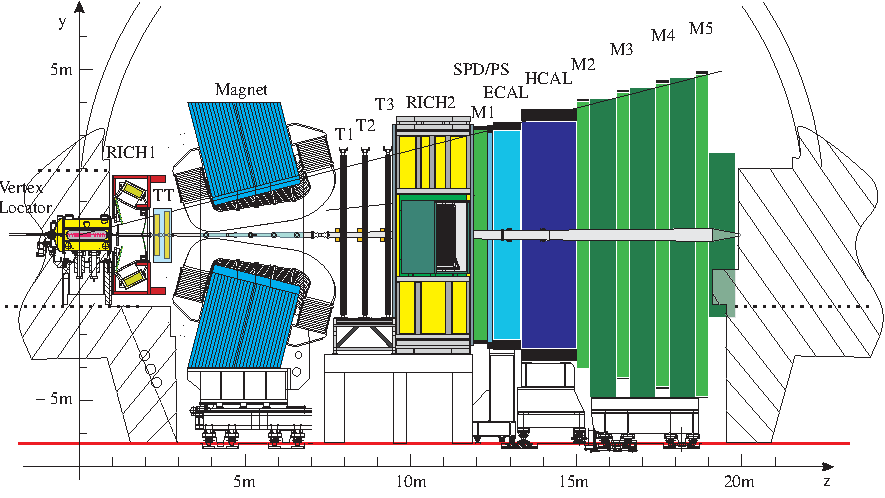
\includegraphics[width=0.95\textwidth]{./figs-detector/lhcb_detector_view.pdf}
    \caption{The LHCb detector.}
    \label{fig:lhcb-detector}
\end{figure}

\begin{figure}[!htb]
    \centering
    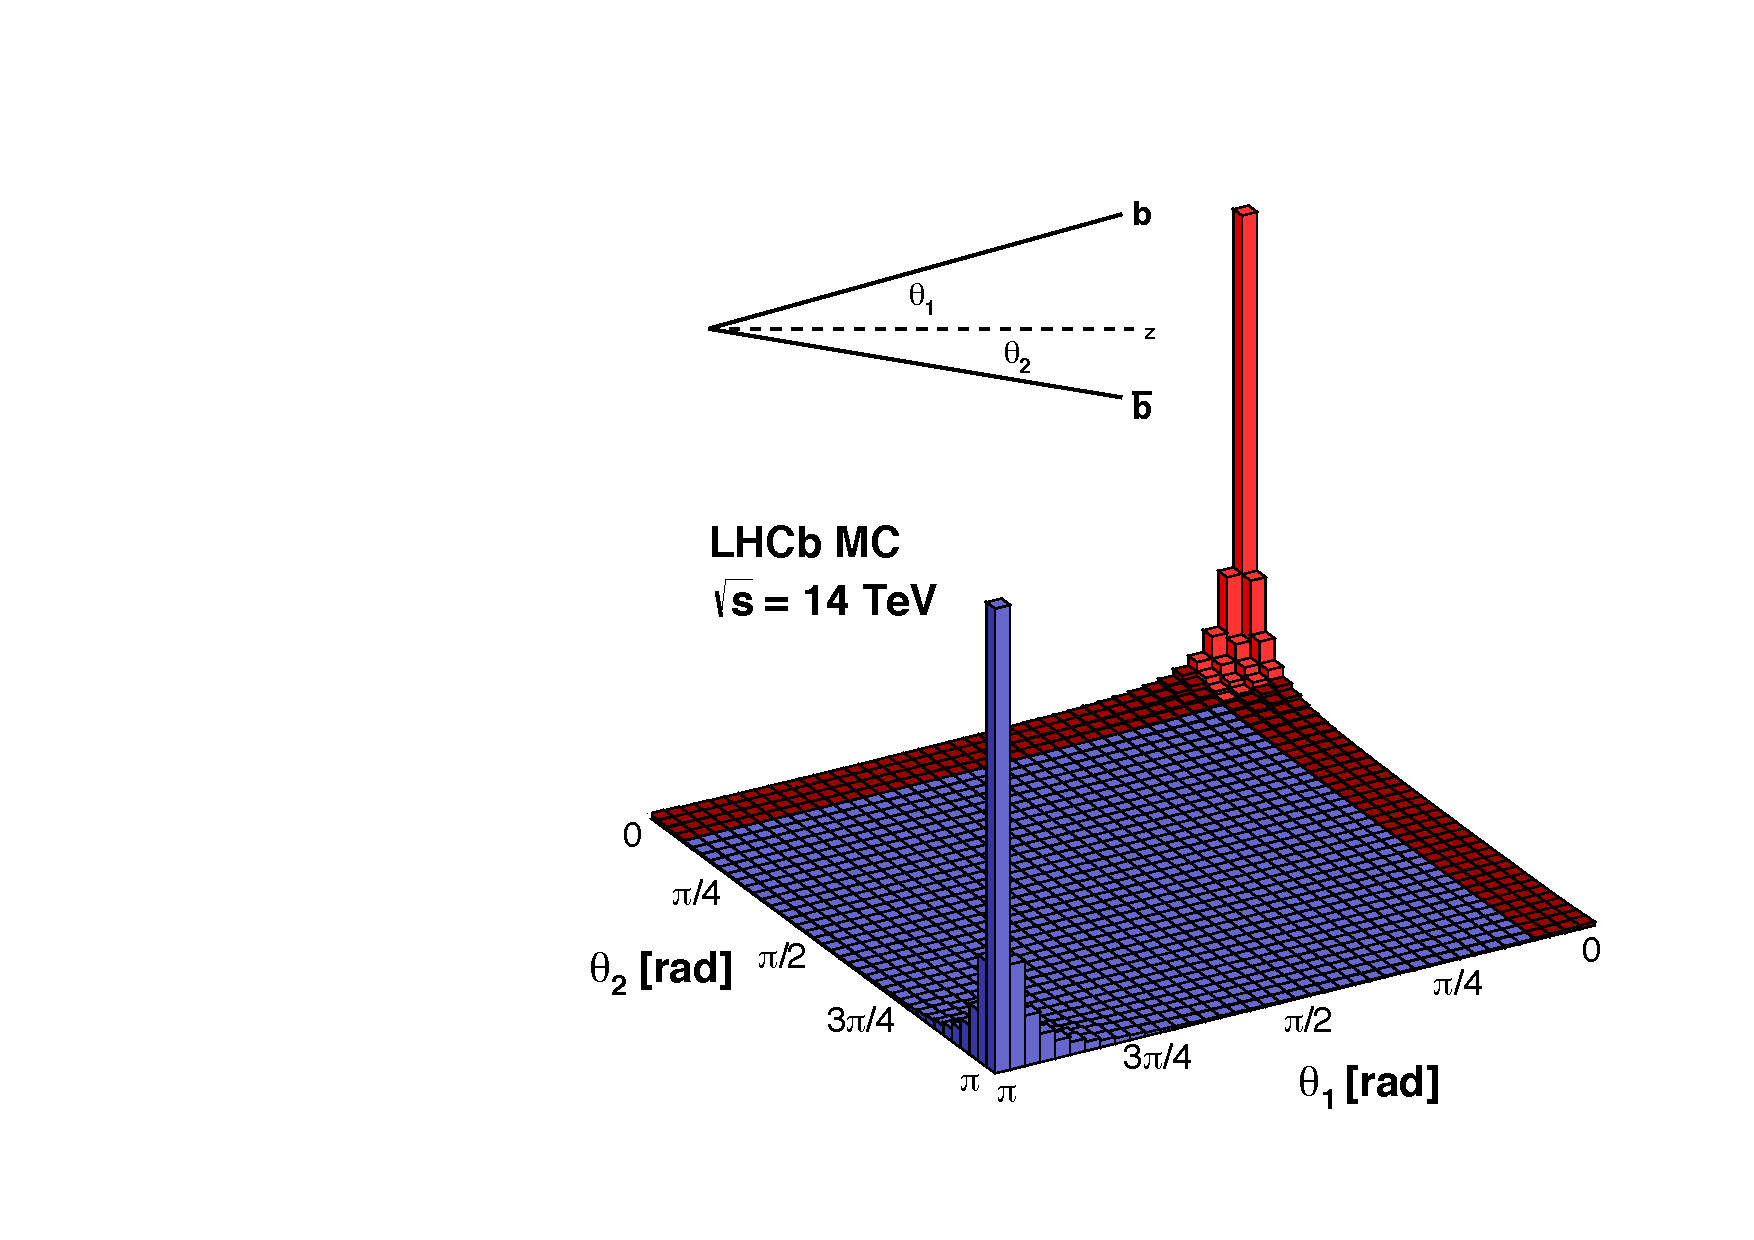
\includegraphics[width=0.6\textwidth]{./figs-detector/14_rad_acc_scheme_right.pdf}
    \caption{
        Simulated \bbbar production angular distribution at $\sqrt{s} = 14$ GeV.
        Taken from \cite{LHCb_bb_prod_angle}.
    }
    \label{fig:bbbar-prod-angular}
\end{figure}


